\begin{figure}
    \captionsetup[subfigure]{labelformat=empty} % stop subcaption writing "(a)""
    \captionsetup{subrefformat=parens} % add parentheses to \subref
    \begin{subfigure}[t]{0.33\columnwidth}
        \inlinelabel{a}{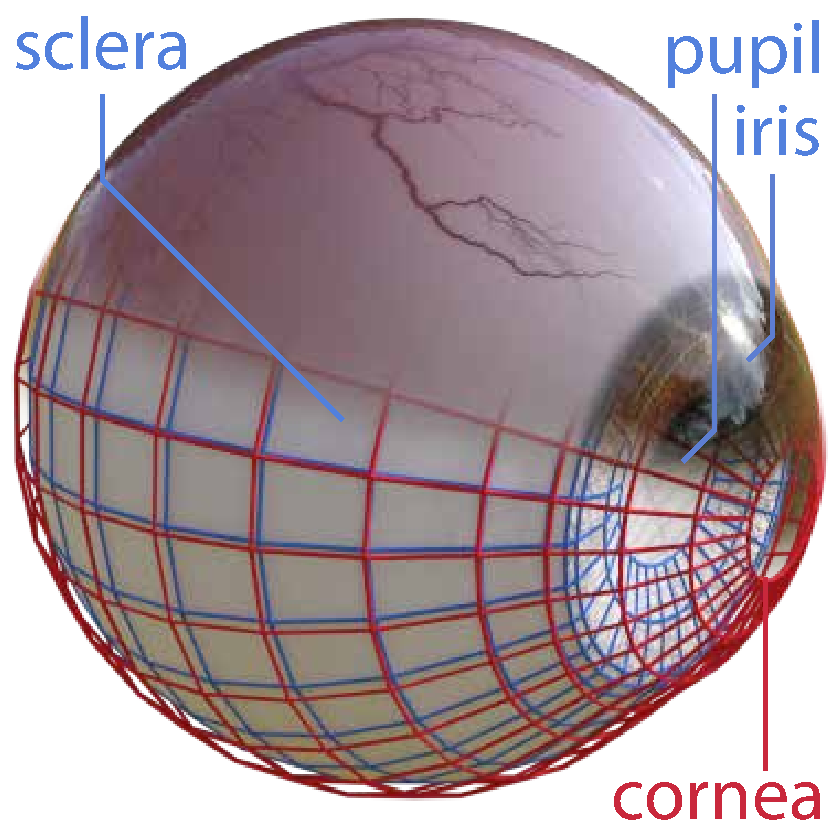
\includegraphics[width=\textwidth]{eye_model}}
        \caption{}\label{fig:eye_model_parts}
    \end{subfigure}
    \hfill
    \begin{subfigure}[t]{0.65\columnwidth}
        \inlinelabel{b}{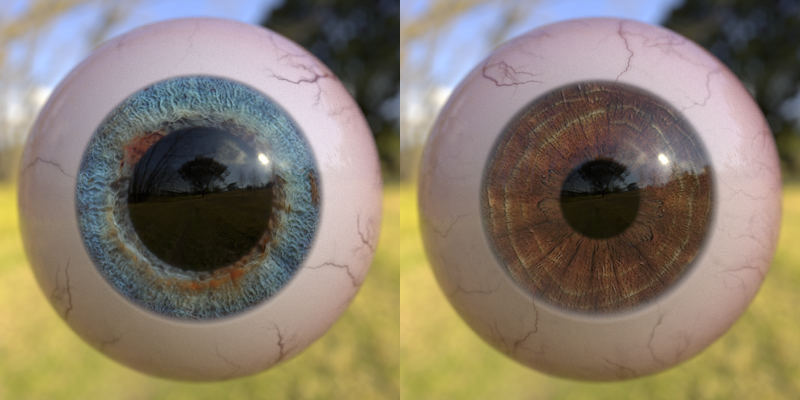
\includegraphics[width=\textwidth]{eye_examples}}
        \caption{}\label{fig:eye_model_images}
    \end{subfigure}
    \par\vspace{-28pt}
    \caption{Our eye model includes the sclera, pupil, iris, and cornea \subref{fig:eye_model_parts} and can exhibit realistic variation in both shape (pupillary dilation) and texture (iris color, scleral veins) \subref{fig:eye_model_images}.}
    \label{fig:eye_model}
\end{figure}